% ============================================================
%  QVF-Hybrid — final narrative deck (GSoC 2026, ML4SCI / DeepLense QML)
%  Rewritten 2026-07-25 to match the final paper (QVF_PAPER.tex).
%  Every number traces to docs/EXPERIMENTS_MASTER.md / the audited paper tables.
% ============================================================
\documentclass[aspectratio=169,10pt]{beamer}
\usetheme{metropolis}
\usepackage{booktabs}
\usepackage{amsmath}
\usepackage{graphicx}

\definecolor{q}{RGB}{217,119,6}
\definecolor{c}{RGB}{37,99,235}
\definecolor{good}{RGB}{22,163,74}
\definecolor{bad}{RGB}{220,38,38}
\newcommand{\gd}[1]{\textcolor{good}{#1}}
\newcommand{\bd}[1]{\textcolor{bad}{#1}}
\newcommand{\qq}[1]{\textcolor{q}{#1}}

\title{QVF-Hybrid: A Guaranteed-Floor Hybrid Quantum--Classical Architecture}
\subtitle{Rigorous controls and an honest paradigm comparison on DeepLense}
\author{GSoC 2026 --- ML4SCI / DeepLense (QML)}
\date{\today}

\begin{document}
\maketitle

% ---------------------------------------------------------------
\begin{frame}{The contribution in one slide}
We built the strongest hybrid we could for the quantum side, ran it through a
\textbf{complete control ladder}, and report exactly what survives.
\smallskip

\scriptsize
\begin{tabular}{@{}llp{6.6cm}@{}}
\toprule
Tier & Control & Verdict \\
\midrule
\textbf{Module} & vs.\ matched \emph{sham} &
  \gd{significant} at (II,\,250): $n{=}20$, $p{=}0.0032<\alpha{=}0.01$;
  small ($+1.4\%$, under our $3\%$ practical bar) \\[1pt]
\textbf{Model} & vs.\ \emph{plain CNN} &
  \gd{guaranteed floor by construction}; vs.-plain contrast
  \bd{not significant} ($p{=}0.088$) \\[1pt]
\textbf{Paradigm} & vs.\ \emph{MAE-ViT} &
  \gd{significant} (Holm $p{=}0.003$, $10/10$, $+22$--$28$\,pp),
  $1/19$ params, \emph{zero} pretraining data \\
\bottomrule
\end{tabular}
\normalsize
\smallskip

\alert{We do \emph{not} claim quantum advantage.}
\end{frame}

% ---------------------------------------------------------------
\begin{frame}{The problem: a baseline crisis in QML}
Published hybrid quantum--classical wins routinely evaporate once the classical
control is made honest.
\smallskip

\begin{itemize}
\item \textbf{Bowles et al.\ 2024}: many hybrid QNNs lose to \emph{trivially small}
      classical baselines once architecture and parameters are matched.
\item \textbf{Schnabel et al.\ 2025} ($\sim$20\,000 models): no robust quantum edge.
\item Our companion QOVT study: orthogonal (RBS) attention \emph{matches but does
      not beat} classical multi-head attention.
\end{itemize}
\smallskip

\begin{alertblock}{Two failure modes}
The quantum model is compared against either (i) a much \textbf{larger} classical
model, or (ii) a \textbf{handicapped sham} whose deficit the circuit merely recovers.
\end{alertblock}

\textbf{Our response:} a control \emph{ladder} --- sham \emph{and} null baseline
\emph{and} multi-seed \emph{and} pre-registration.
\end{frame}

% ---------------------------------------------------------------
\begin{frame}{Task and data}
\textbf{Task.} Classify $64\times64$ lensing images: \qq{axion} (vortex) /
\textbf{CDM} (subhalos) / \textbf{no\_sub} (smooth).
3-class macro-OVR AUC, 9:1 split, best-val-AUC checkpoint.
\smallskip

\footnotesize
\begin{tabular}{@{}lll@{}}
\toprule
Dataset & Character & Role \\
\midrule
Model\_I   & lower SNR, ceiling $\approx0.97$ & second dataset \\
Model\_II  & higher SNR, ceiling $\approx0.99$ & \textbf{primary signal dataset} \\
Model\_III & higher-SNR sibling & generalization check \\
CommonTest & GoogleSC vort/sphere/no & out-of-family \emph{hard case} \\
\bottomrule
\end{tabular}
\normalsize
\smallskip

\textbf{The regime that matters.} LSST / Euclid / Roman give many \emph{unlabeled}
images but few \emph{labeled} ones. We test down to $N{=}100$/class --- where the
classical SOTA is weakest.
\smallskip

\textbf{Target.} MAE-pretrained ViT, AUC $0.968$ (arXiv:2512.06642);
our protocol-matched reproduction $0.9895$ (Model\_II, full data).
\end{frame}

% ---------------------------------------------------------------
\begin{frame}{Evolution (1): QVF-Scratch --- and its apparent win}
CNN $\to$ \emph{Neural Amplitude Encoding} $\to$ 8-qubit
\texttt{StronglyEntanglingLayers} ($T{=}96$) $\to \langle Z\rangle \to$ linear head.
End-to-end, no pretraining.
\smallskip

\footnotesize
\begin{tabular}{@{}lcccc@{}}
\toprule
Dataset & \qq{Quantum} (142.8k) & Sham (144.8k) & MAE-ViT (2.72M) & Q$-$Sham \\
\midrule
Model\_I  & \gd{0.9805} & 0.9790 & 0.9778 & $+0.0015$ \\
Model\_II & \gd{0.9983} & 0.9928 & 0.9895 & $+0.0055$ \\
Dataset1  & \gd{0.9983} & 0.9960 & 0.9895 & $+0.0023$ \\
\bottomrule
\end{tabular}
\normalsize
\smallskip

Plus an 11-point sweep (single seed): quantum $>$ sham at \textbf{21 of 22} points,
peak $\Delta{=}{+}0.112$ at $N{=}1500$.

\begin{alertblock}{But this is what the literature warns about}
A favourable comparison against a \textbf{handicapped sham} and an
\textbf{oversized ViT}. What about a plain CNN?
\end{alertblock}
\end{frame}

% ---------------------------------------------------------------
\begin{frame}{Evolution (2): the null baseline demolishes it}
The missing control: a \emph{plain CNN with direct readout} --- same encoder, same
protocol, \textbf{fewer} params (\textbf{93{,}763}, smallest in the program).
\smallskip

\footnotesize
\textbf{Bottleneck-tax ledger} (Model\_II, $N{=}500$):

\begin{tabular}{@{}lcc@{}}
\toprule
Arm & AUC & vs.\ plain-lin \\
\midrule
plain-lin (un-taxed CNN, 93.8k) & \gd{0.9129} & --- \\
QVF-scratch \qq{quantum} (forced 8-dim readout) & 0.8206 & \bd{$-0.092$} (\textbf{tax}) \\
QVF-scratch sham (forced linear readout) & 0.7683 & \bd{$-0.145$} \\
\midrule
\emph{recovery} (quantum $-$ sham, in bottleneck) & \multicolumn{2}{c}{$+0.052$} \\
\emph{net} (quantum $-$ plain-lin) & \multicolumn{2}{c}{\bd{$-0.092$}} \\
\bottomrule
\end{tabular}
\normalsize
\smallskip

\begin{alertblock}{Reading}
The 8-dim bottleneck is a \textbf{handicap, not a regulariser} --- it loses even at
$N{=}500$. The ``21/22 win'' was measured \emph{inside} a family a plain CNN dominates.
\end{alertblock}
\end{frame}

% ---------------------------------------------------------------
\begin{frame}{Evolution (3): Wide is not enough $\Rightarrow$ Hybrid}
\footnotesize
\textbf{QVF-Wide}: readout $8\to52$ observables
($\langle Z\rangle,\langle X\rangle,\langle Y\rangle,\langle Z_iZ_j\rangle$):

\begin{tabular}{@{}rcccc@{}}
\toprule
$N$ (Model\_II) & wide-Q (52) & wide-sham & orig-Q (8) & plain-lin \\
\midrule
500  & 0.8450 & 0.7850 & 0.8206 & \gd{0.9129} \\
3000 & \bd{0.9631} & 0.9575 & 0.9808 & \gd{0.9849} \\
8000 & 0.9861 & \bd{0.9906} & 0.9896 & \gd{0.9942} \\
\bottomrule
\end{tabular}
\normalsize
\smallskip

\bd{Regresses at mid-$N$}; \bd{sham wins at $N{=}8000$}. Width is not the fix ---
\emph{forcing all 128 CNN dims through the circuit} is the tax.

\begin{block}{QVF-Hybrid: the quantum branch \emph{in residual}}
\vspace{-4pt}
\[
  \hat{y} = W_{\mathrm{head}}\;
  \mathrm{concat}\big(\mathrm{LN}(\mathbf{h}),\,\mathrm{LN}(\mathbf{m})\big) + b
\]
\vspace{-10pt}

Zeroing the $\mathbf{m}$-block reduces \textbf{exactly} to plain-lin (verified,
error $=0.0$) $\Rightarrow$ \gd{plain-CNN floor holds by construction}.
\end{block}
\end{frame}

% ---------------------------------------------------------------
\begin{frame}{The control protocol (fixed before the runs)}
\begin{itemize}
\item \textbf{Capacity-matched sham.} Circuit $\to$ \texttt{Linear+Tanh}; sham always
      has \emph{more} params (156{,}923 vs \textbf{143{,}655}).
\item \textbf{Null baseline.} plain-lin (93{,}763), plain-mlp (142{,}837) ---
      \emph{smaller} than the quantum model.
\item \textbf{Bit-identical subsampling.} Same RNG across methods $\Rightarrow$ every
      arm sees \emph{exactly} the same images per seed.
\item \textbf{Best-val-AUC} checkpoint, never the last epoch.
\item \textbf{Multi-seed}, seed-\emph{paired} (3 seeds; 10--20 for significance).
\item \textbf{Practical bar}: $<3\%$ AUC is not claimed as an effect.
\item \textbf{Pre-registration}: success criteria fixed \emph{before} launch.
\end{itemize}
\smallskip

\footnotesize
MAE-ViT gets its \emph{full} recipe: mask-0.9 pretraining on unlabeled
\texttt{no\_sub}, Adam $5{\times}10^{-5}$, 50 epochs, rot90/flip augmentation.
\end{frame}

% ---------------------------------------------------------------
\begin{frame}{Main result --- three datasets, three paradigms}
\centering
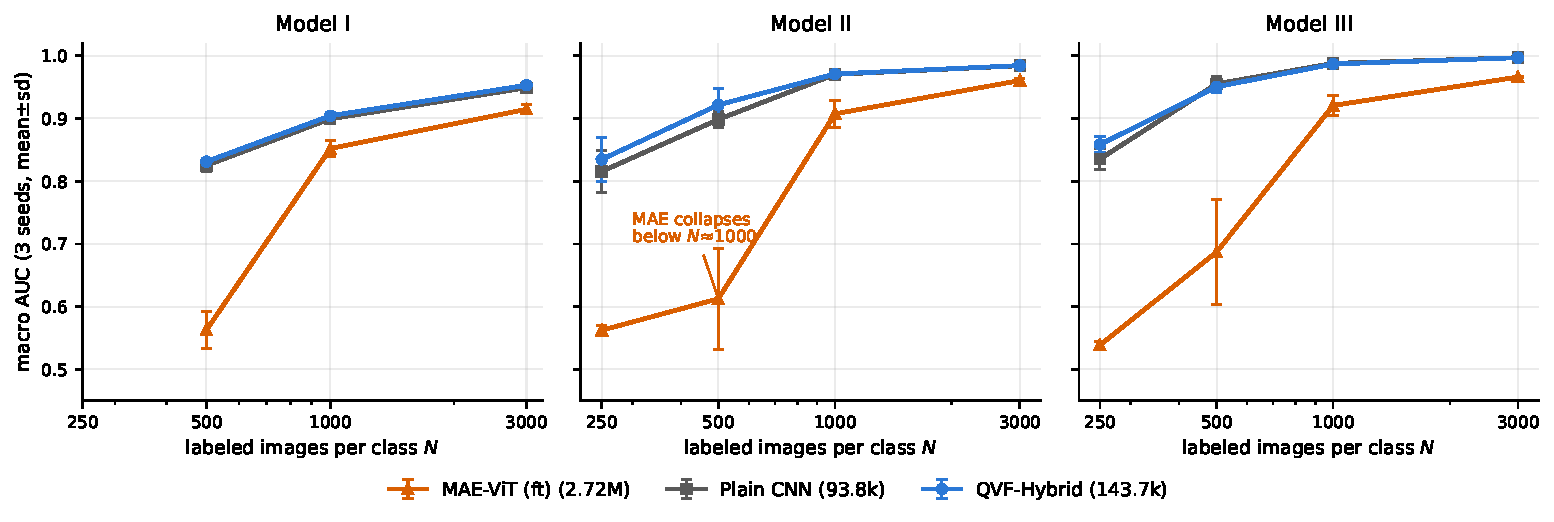
\includegraphics[width=0.93\textwidth]{../figures/hybrid_vs_baselines.pdf}
\\[1pt]
{\scriptsize Macro-OVR AUC vs.\ labeled samples/class, 3 seeds (mean $\pm$ s.d.).
\textbf{QVF-Hybrid} (143.7k, no pretraining) tracks or leads the plain-CNN family
everywhere; \textbf{MAE-ViT} (2.72M, full pretraining $+$ aug $+$ $2.5\times$ epochs)
\bd{collapses below $N\approx1000$}.}
\end{frame}

% ---------------------------------------------------------------
\begin{frame}{The significance battle (two-stage, pre-registered)}
\scriptsize
\textbf{Stage 1} --- all cells, $n{=}10$, Holm over 6 tests:

\begin{tabular}{@{}llcccl@{}}
\toprule
Cell & contrast & pos & mean $\Delta$ & $p$ raw & $p$ Holm \\
\midrule
Model\_II $N{=}250$ & Q$>$plain & 7/10 & $+0.0153$ & 0.032 & 0.161 \;n.s. \\
Model\_II $N{=}250$ & Q$>$sham  & 8/10 & $+0.0189$ & 0.0098 & \emph{0.059 marginal} \\
Model\_II $N{=}500$ & Q$>$plain & 7/10 & $+0.0096$ & 0.077 & 0.309 \;n.s. \\
Model\_II $N{=}500$ & Q$>$sham  & 4/10 & $+0.0017$ & 0.539 & 1.000 \;n.s. \\
Model\_I  $N{=}500$ & Q$>$plain & 6/10 & $+0.0009$ & 0.237 & 0.712 \;n.s. \\
Model\_I  $N{=}500$ & Q$>$sham  & 5/10 & $-0.0010$ & 0.615 & 1.000 \;n.s. \\
\bottomrule
\end{tabular}
\smallskip

\textbf{Stage 2} --- pre-registered sequential confirmation, $n{=}20$, $\alpha{=}0.01$:

\begin{tabular}{@{}llcccl@{}}
\toprule
Cell & contrast & pos & mean $\Delta$ [95\% CI] & $p$ & verdict \\
\midrule
Model\_II $N{=}250$ & Q$>$sham  & 15/20 & $+0.0140$ $[+0.0048,+0.0233]$ & \gd{\textbf{0.0032}} & \gd{\textbf{significant}} \\
Model\_II $N{=}250$ & Q$>$plain & 11/20 & $+0.0081$ $[-0.0010,+0.0172]$ & 0.088 & n.s. \\
\bottomrule
\end{tabular}
\smallskip

\normalsize
\footnotesize
\gd{Module-level significant} vs.\ sham --- but \textbf{sub-3\%}, \textbf{single-cell},
and vs.-plain is \textbf{n.s.} Sequential design disclosed; $\alpha$ fixed before Stage 2.
\end{frame}

% ---------------------------------------------------------------
\begin{frame}{Mechanism: entanglement is compensation, not information}
\footnotesize
\textbf{Forced-readout}: entanglement is load-bearing ---
\gd{ENT $>$ NOENT $>$ SHAM in 6/6 cells}; at the peak cell (II,\,1500) it carries
$\approx$66\% of the quantum-over-sham margin.
\smallskip

\textbf{Residual (hybrid)}, $n{=}10$:

\begin{tabular}{@{}lccccc@{}}
\toprule
$N$ (Model\_II) & ENT & NOENT (Rot only) & SHAM & plain-lin & ENT$-$NOENT \\
\midrule
250 & $0.8339$ & $0.8317$ & $0.8149$ & $0.8186$ & $+0.0022$ ($p{=}0.22$) \\
500 & $0.9198$ & $0.9198$ & $0.9181$ & $0.9102$ & $-0.0000$ ($p{=}0.47$) \\
\bottomrule
\end{tabular}
\normalsize
\smallskip

\begin{alertblock}{Data-processing inequality}
$\mathbf{m}=g(\mathbf{h})$ is deterministic $\Rightarrow
I(Y;(\mathbf{h},\mathbf{m}))=I(Y;\mathbf{h})$:
\textbf{the branch cannot add label information}, only reshape geometry.
\end{alertblock}

\footnotesize
Peak margin (II,\,1500): \textbf{$+0.108$ forced} $\to$ \textbf{$+0.001$ hybrid}
--- a $100\times$ collapse. Entanglement mattered only while the architecture was crippled.
\end{frame}

% ---------------------------------------------------------------
\begin{frame}{Paradigm duel: QVF-Hybrid vs.\ MAE-ViT}
\scriptsize
\begin{tabular}{@{}llccccl@{}}
\toprule
Data & $N$ & QVF-Hybrid & MAE-ft & $\Delta$ & plain-lin & verdict \\
\midrule
Model\_II & 250  & \gd{0.8347} & 0.5623 & \gd{$+0.272$} & 0.8155 & \gd{PASS 3/3} \\
Model\_II & 500  & \gd{0.9216} & 0.6125 & \gd{$+0.309$} & 0.8984 & \gd{PASS 3/3} \\
Model\_II & 1000 & \gd{0.9709} & 0.9074 & \gd{$+0.064$} & 0.9702 & \gd{PASS 3/3} \\
Model\_II & 3000 & 0.9843 & 0.9604 & $+0.024$ & 0.9841 & \bd{$\times$ ($<3\%$)} \\
Model\_I  & 500  & \gd{0.8312} & 0.5627 & \gd{$+0.269$} & 0.8252 & \gd{PASS 3/3} \\
Model\_I  & 1000 & \gd{0.9043} & 0.8520 & \gd{$+0.052$} & 0.8993 & \gd{PASS 3/3} \\
Model\_I  & 3000 & \gd{0.9530} & 0.9147 & \gd{$+0.038$} & 0.9490 & \gd{PASS 3/3} \\
\bottomrule
\end{tabular}
\normalsize
\smallskip

\footnotesize
\textbf{Scoreboard:} \gd{10 of 11 cells} across three datasets clear the
pre-registered $\geq3\%$ bar ($+3.1$ to $+32.0$\,pp).
\textbf{Significance:} \gd{Holm $p{=}0.003$, $10/10$, $+22$--$28$\,pp} on three
low-$N$ cells. \textbf{MAE-probe} (frozen $+$ linear): $0.49$--$0.51$, \bd{random-level}.

\begin{alertblock}{Honest attribution}
The win belongs to the \textbf{CNN inductive-bias family}, not the circuit ---
plain-lin also crushes MAE-ft (II,\,500: $0.8984$ vs $0.6125$).
QVF-Hybrid is the best \emph{variant} of that family on Model\_II.
\end{alertblock}
\end{frame}

% ---------------------------------------------------------------
\begin{frame}{Negative results (honesty is the product)}
\footnotesize
\begin{tabular}{@{}lp{7.6cm}@{}}
\toprule
Lever & Outcome \\
\midrule
Wide readout (52 obs.) & \bd{regresses} at mid-$N$; sham wins at $N{=}8000$ \\
Qubit scaling $8\to12$ & \bd{does not transfer}: (II,500) identical
  ($0.9216{=}0.9216$); on Model\_I the nq12 \emph{sham} (0.8471) \bd{beats} quantum
  (0.8387); params balloon to 639k \\
Circuit LR ($10^{-2}$) & \bd{inert} (0.9188 vs 0.9216) \\
TDA (persistent homology) & \bd{all 3 criteria failed}; the pairing-broken null
  \emph{matches} real features $\Rightarrow$ no topological label information \\
QMAE (raw-pixel amplitude) & \bd{sham wins everywhere} ($-0.012$ to $-0.050$)
  across $L{=}3{\to}20$, res $16{\to}64$, $N_Q{=}12{\to}14$ \\
Angle enc., Model\_III full & \bd{unstable} (AUC oscillates 0.27--0.61) \\
\bottomrule
\end{tabular}
\normalsize
\smallskip

The old ``more qubits $\Rightarrow$ bigger quantum win'' law was \emph{bottleneck
compensation}: remove the bottleneck and the lever dies --- exactly what DPI predicts.
\end{frame}

% ---------------------------------------------------------------
\begin{frame}{Generalization: a third dataset and a hard case}
\footnotesize
\textbf{Model\_III} (3 seeds):

\begin{tabular}{@{}rccccc@{}}
\toprule
$N$ & hyb-Q & hyb-sham & plain-lin & MAE-ft & $\Delta$ vs.\ MAE \\
\midrule
250  & \gd{0.8585} & 0.8314 & 0.8353 & 0.5387 & \gd{$+0.320$} \\
500  & 0.9504 & 0.9460 & \gd{0.9551} & 0.6868 & \gd{$+0.264$} \\
1000 & 0.9867 & 0.9856 & \gd{0.9879} & 0.9207 & \gd{$+0.066$} \\
3000 & 0.9968 & 0.9968 & \gd{0.9969} & 0.9660 & \gd{$+0.031$} \\
\bottomrule
\end{tabular}
\smallskip

At (III,\,250): Q$>$sham $+0.027$ (3/3 seed-paired) --- low-$N$ direction
\gd{replicates on a third dataset} ($n{=}3$, no significance claim).
All four cells clear the $\geq3\%$ paradigm bar.
\smallskip

\textbf{CommonTest} (hard case, 80 ep, full data): plain-mlp $0.8087$ /
plain-lin $0.7951$ / hyb-S $0.8025$ / hyb-Q $0.7968$ / \bd{MAE-ft $0.6207$}.
\normalsize
\smallskip

\footnotesize
\begin{itemize}
\item Paradigm ordering \gd{reproduces}: CNN family $\gg$ MAE-ft.
\item Hybrid \gd{floor holds}; quantum $\approx$ sham --- the low-$N$ gain lives in
      a regime CommonTest never reaches.
\end{itemize}
\end{frame}

% ---------------------------------------------------------------
\begin{frame}{Conclusion --- the three-tier claim ladder}
\footnotesize
\begin{enumerate}
\item \textbf{Module} (circuit vs.\ matched sham): \gd{statistically significant} at
      (II,\,250), pre-registered two-stage design ($n{=}20$, $p{=}0.0032<\alpha{=}0.01$).
      Magnitude $+1.4\%$ --- \alert{below our 3\% practical bar}. Driven by
      amplitude-embedding structure, \textbf{not} entanglement.
\item \textbf{Model} (vs.\ plain CNN): \gd{guaranteed floor by construction};
      vs.-plain \bd{not significant} ($p{=}0.088$) $\Rightarrow$ no model-level claim.
\item \textbf{Paradigm} (vs.\ MAE-ViT): \gd{significant} (Holm $p{=}0.003$, $10/10$,
      $+22$--$28$\,pp), $10/11$ cells over the bar across three datasets, $1/19$ params,
      \textbf{zero} pretraining data --- credit to the \textbf{CNN family}.
\end{enumerate}
\normalsize
\smallskip

\begin{alertblock}{The honest headline}
\textbf{We do not claim quantum advantage.} We claim a significance-tested
\emph{module-level} contribution too small to justify quantum hardware on this task
--- plus a mechanism (DPI) explaining why it cannot be larger, and the negative
results that bound it.
\end{alertblock}
\end{frame}

% ---------------------------------------------------------------
\begin{frame}[standout]
Paper, code, figures, and every number:\\[4pt]
\small github.com/leo07010/gsoc2026-deeplense-qml
\end{frame}

\end{document}
